\chapter{The Two-Body Problem}
\label{ch:two_body_problem}

\section{Introduction to the Two-Body Problem}

The \textbf{two-body problem} is the foundation of orbital mechanics. It describes the motion of two point masses interacting only through mutual gravitational attraction. This is the only case in celestial mechanics with a complete analytical solution.

\subsection{Problem Statement}

Consider two bodies with masses $m_1$ and $m_2$ separated by distance $r$. Newton's law of gravitation gives:

\begin{equation}
    \mathbf{F}_{12} = -G\frac{m_1 m_2}{r^2}\hat{\mathbf{r}}
\end{equation}

where $G = 6.674 \times 10^{-11}$ m$^3$ kg$^{-1}$ s$^{-2}$ is the gravitational constant.

The equations of motion are:
\begin{align}
    m_1\ddot{\mathbf{r}}_1 &= G\frac{m_1 m_2}{r^3}(\mathbf{r}_2 - \mathbf{r}_1) \\
    m_2\ddot{\mathbf{r}}_2 &= G\frac{m_1 m_2}{r^3}(\mathbf{r}_1 - \mathbf{r}_2)
\end{align}

\subsection{Reduction to One-Body Problem}

By introducing the relative position $\mathbf{r} = \mathbf{r}_2 - \mathbf{r}_1$ and the reduced mass $\mu = G(m_1 + m_2)$, the problem reduces to:

\begin{equation}
    \ddot{\mathbf{r}} = -\frac{\mu}{r^3}\mathbf{r}
\end{equation}

This is the \textbf{central force equation} with gravitational parameter $\mu$. For the Sun-planet system, $\mu_\odot = 1.327 \times 10^{20}$ m$^3$ s$^{-2}$.

\section{Conservation Laws}

The two-body problem has several conserved quantities that constrain the motion.

\subsection{Conservation of Angular Momentum}

The angular momentum is:
\begin{equation}
    \mathbf{h} = \mathbf{r} \times \mathbf{v}
\end{equation}

Since $\ddot{\mathbf{r}}$ is parallel to $\mathbf{r}$, we have:
\begin{equation}
    \frac{d\mathbf{h}}{dt} = \mathbf{r} \times \ddot{\mathbf{r}} = \mathbf{0}
\end{equation}

Therefore: $\mathbf{h} = \text{constant}$

\textbf{Consequences}:
\begin{itemize}
    \item Motion is confined to a plane perpendicular to $\mathbf{h}$
    \item $|\mathbf{h}| = h = \sqrt{\mu a(1-e^2)}$ relates to orbital elements
    \item Areal velocity is constant: $\frac{dA}{dt} = \frac{h}{2}$ (Kepler's Second Law)
\end{itemize}

\subsection{Conservation of Energy}

The specific mechanical energy is:
\begin{equation}
    \mathcal{E} = \frac{v^2}{2} - \frac{\mu}{r} = \text{constant}
\end{equation}

This can be written as:
\begin{equation}
    \mathcal{E} = -\frac{\mu}{2a}
\end{equation}

for elliptical orbits with semi-major axis $a$.

\subsection{The Laplace-Runge-Lenz Vector}

The eccentricity vector is conserved:
\begin{equation}
    \mathbf{e} = \frac{1}{\mu}(\mathbf{v} \times \mathbf{h}) - \frac{\mathbf{r}}{r}
\end{equation}

Properties:
\begin{itemize}
    \item $|\mathbf{e}| = e$ (orbital eccentricity)
    \item $\mathbf{e}$ points toward periapsis
    \item $\mathbf{e} \cdot \mathbf{h} = 0$ (perpendicular to angular momentum)
\end{itemize}

\section{The Orbit Equation}

\subsection{Derivation}

In polar coordinates $(r, \nu)$ where $\nu$ is the true anomaly, the orbit equation is:

\begin{equation}
    r = \frac{a(1-e^2)}{1 + e\cos\nu} = \frac{p}{1 + e\cos\nu}
\end{equation}

where $p = a(1-e^2)$ is the semi-latus rectum.

This is the equation of a conic section with focus at the origin.

\subsection{Conic Sections}

The orbit shape depends on eccentricity and energy:

\begin{figure}[htbp]
\centering
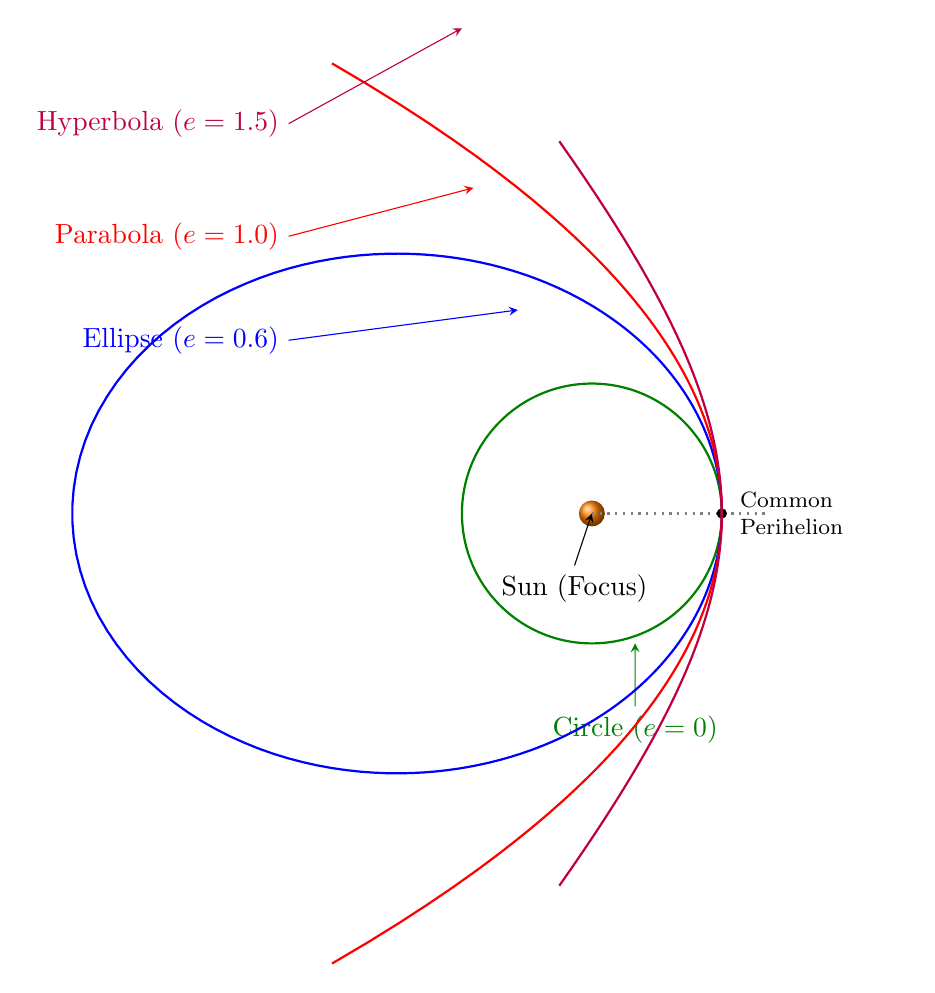
\begin{tikzpicture}[scale=1.1, >=stealth]
    % PARAMETRI
    \def\q{1.5} % Distanza Perielio comune
    
    % 1. SOLE (Focus)
    \coordinate (Sun) at (0,0);
    \shade[ball color=orange] (Sun) circle (0.15);
    \draw[<-] (Sun) -- ++(-0.2, -0.6) node[below] {Sun (Focus)};

    % 2. LINEA PERIELIO (Common Perihelion)
    \draw[dotted, gray, thick] (0,0) -- (\q+0.5, 0);
    \filldraw[black] (\q, 0) circle (1.5pt);
    \node[right, font=\footnotesize, text width=2cm] at (\q+0.1, 0) {Common\\Perihelion};

    % 3. CERCHIO (e=0)
    \draw[thick, green!50!black] (0,0) circle (\q);
    % Etichetta: Basso
    \node[green!50!black] (circle_label) at (0.5, -2.5) {Circle ($e=0$)};
    \draw[->, green!50!black, thin] (circle_label) -- (0.5, -\q);

    % 4. ELLISSE (e=0.6)
    \draw[thick, blue, samples=200, domain=0:360] plot ({\x}:{2.4/(1+0.6*cos(\x))});
    % Etichetta: Sinistra Alto
    \node[blue, anchor=east] (ellipse_label) at (-3.5, 2.0) {Ellipse ($e=0.6$)};
    \draw[->, blue, thin] (ellipse_label.east) -- (110:2.5);

    % 5. PARABOLA (e=1.0)
    \draw[thick, red, samples=100, domain=-120:120] plot ({\x}:{3.0/(1+cos(\x))});
    % Etichetta: Sinistra Più Alto
    \node[red, anchor=east] (parabola_label) at (-3.5, 3.2) {Parabola ($e=1.0$)};
    \draw[->, red, thin] (parabola_label.east) -- (110:4.0);

    % 6. IPERBOLE (e=1.5)
    \draw[thick, purple, samples=100, domain=-95:95] plot ({\x}:{3.75/(1+1.5*cos(\x))});
    % Etichetta: Sinistra Altissimo
    \node[purple, anchor=east] (hyperbola_label) at (-3.5, 4.5) {Hyperbola ($e=1.5$)};
    \draw[->, purple, thin] (hyperbola_label.east) -- (105:5.8);

\end{tikzpicture}
\caption{Family of conic orbits sharing a common focus (Sun) and perihelion distance. The eccentricity $e$ determines the "openness" of the orbit.}
\label{fig:conic_sections}
\end{figure}

\begin{table}[htbp]
\centering
\begin{tabular}{lccc}
\toprule
\textbf{Orbit Type} & \textbf{Eccentricity} & \textbf{Energy} & \textbf{Examples} \\
\midrule
Circle & $e = 0$ & $\mathcal{E} < 0$ & Idealized orbits \\
Ellipse & $0 < e < 1$ & $\mathcal{E} < 0$ & Planets, asteroids \\
Parabola & $e = 1$ & $\mathcal{E} = 0$ & Escape trajectory \\
Hyperbola & $e > 1$ & $\mathcal{E} > 0$ & Interstellar objects \\
\bottomrule
\end{tabular}
\caption{Classification of orbital conics by eccentricity and energy.}
\label{tab:orbit_types}
\end{table}

\section{Kepler's Laws}

Johannes Kepler (1571-1630) derived three empirical laws from observations of planetary motion. These are consequences of the two-body problem.

\subsection{Kepler's First Law (Law of Ellipses)}

\textit{The orbit of a planet is an ellipse with the Sun at one focus.}

Mathematically:
\begin{equation}
    r = \frac{a(1-e^2)}{1 + e\cos\nu}
\end{equation}

The perihelion distance is $r_p = a(1-e)$ and aphelion distance is $r_a = a(1+e)$.

\subsection{Kepler's Second Law (Law of Equal Areas)}

\textit{A line joining a planet and the Sun sweeps out equal areas in equal times.}

This follows from conservation of angular momentum:
\begin{equation}
    \frac{dA}{dt} = \frac{h}{2} = \frac{1}{2}\sqrt{\mu a(1-e^2)} = \text{constant}
\end{equation}

\subsection{Kepler's Third Law (Harmonic Law)}

\textit{The square of the orbital period is proportional to the cube of the semi-major axis.}

\begin{equation}
    P^2 = \frac{4\pi^2}{\mu}a^3
\end{equation}

For the solar system:
\begin{equation}
    P[\text{years}] = a[\text{AU}]^{3/2}
\end{equation}

\section{Kepler's Equation}

\subsection{The Anomalies}

Three related angles describe position in an elliptical orbit:

\begin{description}
    \item[True Anomaly ($\nu$)] Actual angle from perihelion to current position
    \item[Eccentric Anomaly ($E$)] Auxiliary angle on the circumscribed circle
    \item[Mean Anomaly ($M$)] Angle that would be covered if motion were uniform
\end{description}

\begin{figure}[htbp]
\centering
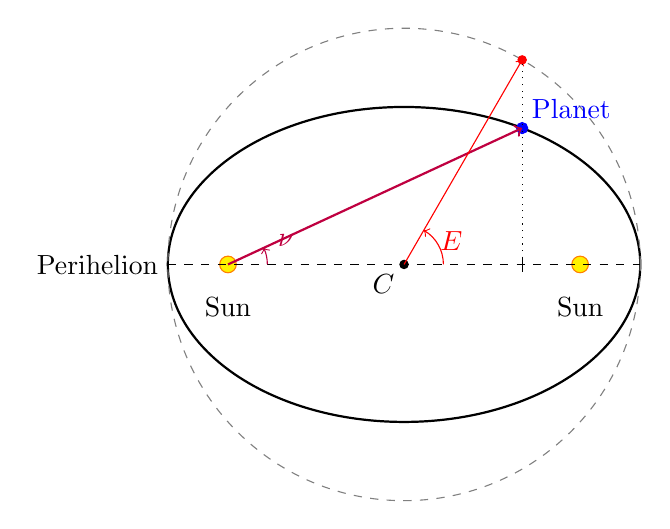
\begin{tikzpicture}[scale=1.0]
    % Ellipse a=3, b=2
    \draw[thick] (0,0) ellipse (3cm and 2cm);
    
    % Circumscribed circle r=3
    \draw[dashed,gray] (0,0) circle (3cm);
    
    % Sun at focus c = sqrt(9-4) = 2.236
    \filldraw[yellow,draw=orange] (2.236,0) circle (3pt);
    \node[below] at (2.236,-0.3) {Sun};
    
    % Center
    \filldraw[black] (0,0) circle (1.5pt);
    \node[below left] at (0,0) {$C$};
    
    % Use x = 1.5
    % y_ell = 2 * sqrt(1 - 0.5^2) = 1.732
    % y_circ = 3 * sqrt(1 - 0.5^2) = 2.598
    
    % Perihelion (right side for positive x focus)
    % Wait, usually nu is measured from Perihelion.
    % If Sun is at right focus (2.236,0), Perihelion is at (3,0).
    % Let's stick to standard: Focus at origin? No, TikZ draws ellipse centered at 0.
    % Let's put Sun at LEFT focus (-2.236,0), Perihelion at (-3,0).
    
    % Sun at LEFT focus
    \filldraw[yellow,draw=orange] (-2.236,0) circle (3pt);
    \node[below] at (-2.236,-0.3) {Sun};
    
    % Perihelion
    \draw[dashed] (-3,0) -- (3,0);
    \node[left] at (-3,0) {Perihelion};
    
    % Planet position at x=1.5, y=1.732
    \filldraw[blue] (1.5,1.732) circle (2pt);
    \node[above right,blue] at (1.5,1.732) {Planet};
    
    % Point on circle (for eccentric anomaly)
    \filldraw[red] (1.5,2.598) circle (1.5pt);
    
    % True anomaly vector (from Sun to Planet)
    \draw[->,purple,thick] (-2.236,0) -- (1.5,1.732);
    % Angle arc
    \draw[->,purple] (-1.736,0) arc (0:25:0.5); 
    \node[purple] at (-1.5,0.3) {$\nu$};
    
    % Eccentric anomaly vector (from Center to Circle Point)
    \draw[->,red] (0,0) -- (1.5,2.598);
    \draw[->,red] (0.5,0) arc (0:60:0.5);
    \node[red] at (0.6,0.3) {$E$};
    
    % Vertical line
    \draw[dotted] (1.5,0) -- (1.5,2.598);
    
    % Label x-axis projection
    \draw (1.5,0.1) -- (1.5,-0.1);
\end{tikzpicture}
\caption{Relationship between true anomaly $\nu$ and eccentric anomaly $E$ in an elliptical orbit.}
\label{fig:anomalies}
\end{figure}

\subsection{Kepler's Equation}

The mean anomaly advances uniformly with time:
\begin{equation}
    M = n(t - t_p) = \sqrt{\frac{\mu}{a^3}}(t - t_p)
\end{equation}

where $t_p$ is the time of perihelion passage and $n$ is the mean motion.

Kepler's equation relates $M$ to $E$:
\begin{equation}
    M = E - e\sin E
\end{equation}

This is a transcendental equation with no closed-form solution. It must be solved iteratively.

\subsection{Solving Kepler's Equation}

\textbf{Newton-Raphson Method}:

Given $M$ and $e$, find $E$ iteratively:
\begin{align}
    f(E) &= E - e\sin E - M = 0 \\
    f'(E) &= 1 - e\cos E \\
    E_{n+1} &= E_n - \frac{f(E_n)}{f'(E_n)} = E_n - \frac{E_n - e\sin E_n - M}{1 - e\cos E_n}
\end{align}

Initial guess: $E_0 = M$ (for small $e$) or $E_0 = M + e$ (better for moderate $e$).

Convergence is typically achieved in 3-5 iterations for $\epsilon < 10^{-12}$.

\subsection{Relationship Between Anomalies}

Once $E$ is known, the true anomaly is:
\begin{equation}
    \nu = 2\arctan\left(\sqrt{\frac{1+e}{1-e}}\tan\frac{E}{2}\right)
\end{equation}

Or equivalently:
\begin{align}
    \cos\nu &= \frac{\cos E - e}{1 - e\cos E} \\
    \sin\nu &= \frac{\sqrt{1-e^2}\sin E}{1 - e\cos E}
\end{align}

The radial distance is:
\begin{equation}
    r = a(1 - e\cos E)
\end{equation}

\section{The Vis-Viva Equation}

The \textbf{vis-viva equation} (``living force'') relates velocity to position:

\begin{equation}
    v^2 = \mu\left(\frac{2}{r} - \frac{1}{a}\right)
\end{equation}

This is derived from energy conservation and is valid for all conic orbits.

\subsection{Special Cases}

\textbf{At perihelion} ($r = a(1-e)$):
\begin{equation}
    v_p = \sqrt{\frac{\mu}{a}\frac{1+e}{1-e}}
\end{equation}

\textbf{At aphelion} ($r = a(1+e)$):
\begin{equation}
    v_a = \sqrt{\frac{\mu}{a}\frac{1-e}{1+e}}
\end{equation}

\textbf{Circular orbit} ($e = 0$, $r = a$):
\begin{equation}
    v_c = \sqrt{\frac{\mu}{a}}
\end{equation}

\textbf{Escape velocity} (parabolic, $e = 1$, $a \to \infty$):
\begin{equation}
    v_e = \sqrt{\frac{2\mu}{r}}
\end{equation}

\section{Parabolic and Hyperbolic Orbits}

\subsection{Parabolic Orbits ($e = 1$)}

For escape trajectories, the orbit equation becomes:
\begin{equation}
    r = \frac{p}{1 + \cos\nu}
\end{equation}

where $p$ is the periapsis distance.

The time-of-flight is given by Barker's equation:
\begin{equation}
    t - t_p = \frac{1}{2}\sqrt{\frac{p^3}{\mu}}\left(\tan\frac{\nu}{2} + \frac{1}{3}\tan^3\frac{\nu}{2}\right)
\end{equation}

\subsection{Hyperbolic Orbits ($e > 1$)}

For interstellar or flyby trajectories:
\begin{equation}
    r = \frac{a(e^2-1)}{1 + e\cos\nu}
\end{equation}

Note: $a < 0$ for hyperbolic orbits (negative energy).

The hyperbolic anomaly $F$ satisfies:
\begin{equation}
    M_h = e\sinh F - F
\end{equation}

And the true anomaly is:
\begin{equation}
    \nu = 2\arctan\left(\sqrt{\frac{e+1}{e-1}}\tanh\frac{F}{2}\right)
\end{equation}

The asymptotic velocity at infinity is:
\begin{equation}
    v_\infty = \sqrt{-\frac{\mu}{a}} = \sqrt{\mu\frac{e^2-1}{a}}
\end{equation}

\section{Lagrange Coefficients}

The \textbf{Lagrange coefficients} (or $f$ and $g$ functions) provide a way to propagate orbits without explicitly computing orbital elements.

\subsection{Definition}

Given initial state $(\mathbf{r}_0, \mathbf{v}_0)$ at time $t_0$, the state at time $t$ is:

\begin{align}
    \mathbf{r}(t) &= f(t)\mathbf{r}_0 + g(t)\mathbf{v}_0 \\
    \mathbf{v}(t) &= \dot{f}(t)\mathbf{r}_0 + \dot{g}(t)\mathbf{v}_0
\end{align}

where $f, g, \dot{f}, \dot{g}$ are scalar functions of time.

\subsection{Expressions for Lagrange Coefficients}

For elliptical orbits:
\begin{align}
    f &= 1 - \frac{a}{r_0}(1 - \cos\Delta E) \\
    g &= t - t_0 + \sqrt{\frac{a^3}{\mu}}(\sin\Delta E - \Delta E) \\
    \dot{f} &= -\sqrt{\frac{\mu a}{rr_0}}\sin\Delta E \\
    \dot{g} &= 1 - \frac{a}{r}(1 - \cos\Delta E)
\end{align}

where $\Delta E = E - E_0$ is the change in eccentric anomaly.

\subsection{Properties}

The Lagrange coefficients satisfy:
\begin{equation}
    f\dot{g} - \dot{f}g = 1
\end{equation}

This is the \textbf{Lagrange identity}, which ensures conservation of the Wronskian.

\section{AstDyn Implementation}

AstDyn provides functions for solving the two-body problem:

\begin{lstlisting}[language=C++,caption={Two-body problem in AstDyn}]
#include <astdyn/dynamics/TwoBody.hpp>
#include <astdyn/core/OrbitalElements.hpp>

using namespace astdyn;

// Solve Kepler's equation
double M = 45.0 * DEG_TO_RAD;  // Mean anomaly
double e = 0.3;                 // Eccentricity
double E = TwoBody::solve_kepler_equation(M, e);
std::cout << "Eccentric anomaly: " << E * RAD_TO_DEG << " deg\n";

// Convert E to true anomaly
double nu = TwoBody::eccentric_to_true_anomaly(E, e);
std::cout << "True anomaly: " << nu * RAD_TO_DEG << " deg\n";

// Compute position and velocity from orbital elements
OrbitalElements kep;
kep.a = 2.5;  // AU
kep.e = 0.15;
kep.M = M;
// ... set other elements

auto [r, v] = kep.to_position_velocity();

// Propagate using Lagrange coefficients
double dt = 100.0;  // days
auto [f, g, fdot, gdot] = TwoBody::lagrange_coefficients(
    r, v, dt, MU_SUN
);

Vector3d r_new = f * r + g * v;
Vector3d v_new = fdot * r + gdot * v;

std::cout << "New position: " << r_new.transpose() << " AU\n";
std::cout << "New velocity: " << v_new.transpose() << " AU/day\n";
\end{lstlisting}

\section{Summary}

Key points about the two-body problem:

\begin{enumerate}
    \item The two-body problem has an \textbf{exact analytical solution}
    \item Motion is governed by conservation of energy, angular momentum, and the eccentricity vector
    \item Orbits are \textbf{conic sections}: circles, ellipses, parabolas, or hyperbolas
    \item \textbf{Kepler's laws} are direct consequences of Newton's gravity
    \item \textbf{Kepler's equation} ($M = E - e\sin E$) relates mean and eccentric anomalies
    \item The \textbf{vis-viva equation} relates velocity to position
    \item \textbf{Lagrange coefficients} enable efficient orbit propagation
\end{enumerate}

Understanding the two-body problem is essential for:
\begin{itemize}
    \item Predicting planetary and asteroid positions
    \item Designing spacecraft trajectories
    \item Understanding the baseline from which perturbations deviate
    \item Developing efficient numerical propagators
\end{itemize}

In the next chapter, we will study perturbations—deviations from the ideal two-body motion caused by additional forces.
